\documentclass[a4paper,11pt]{report}
\usepackage[T1]{fontenc}
\usepackage[utf8]{inputenc}
\usepackage{lmodern}
\usepackage[francais]{babel}
\usepackage{graphicx}
\usepackage{array}

\title{Data wars}
\author{Guillaume LARROYENNE, Nathan PRETOT,\\ Jeremy RENAUD,Tom SALVI, Pierre VALENZA}

\begin{document}

\maketitle
\tableofcontents

\begin{abstract}
\end{abstract}

\chapter{Mise en œuvre}

  \section{Répartition du travail}
    Ce projet mettant en œuvre une grande diversité de domaine (site web, jeu, serveur, base de données, graphisme), nous n'avons donc pas eu d'autres choix que de répartir notre effectif sur les différents domaines. Laissant ainsi presque tout les domaines (à part modèle) couvert par une seule personne, nous laissant la disposition suivante :
    \begin{description}
      \item[Jeremy : ] implémentation des interfaces et des contrôleurs.
      \item[Tom : ] travail sur une partie du modèle du jeu.
      \item[Guillaume :] modélisation et création du serveur et des communications réseaux.
      \item[Pierre :] création du site web.
      \item[Nathan :] modélisation et création de la base de données. Modélisation du jeu et réalisation d'une partie de celui-ci.
    \end{description}
    
    \begin{figure}[th]
      \begin{center}
        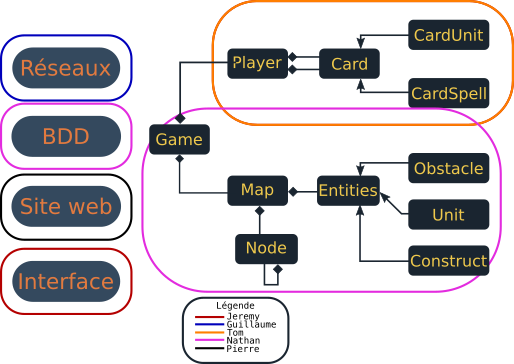
\includegraphics[scale=0.365]{Assets/UMLRepartition.png}
        \caption{Répartition du travail}
        \label{RepTravail}
      \end{center}
    \end{figure}
    
    De plus des éléments du domaine informatiques, notre projet nous a demandé la création entière d'un jeu, nous demandant une réflexion autours des règles et fonctionnalités de celui-ci, ainsi que de créer des cartes innovantes pour celui-ci. Cette partie à été endossée par l'ensemble de l'équipe.
    
  \section{Gestion du temps}
    Le projet a débuté sur la conception du jeu. C'est-à-dire la création des règles, ainsi que les éléments de modélisation a au niveau
    \begin{figure}[th]
      \begin{center}
        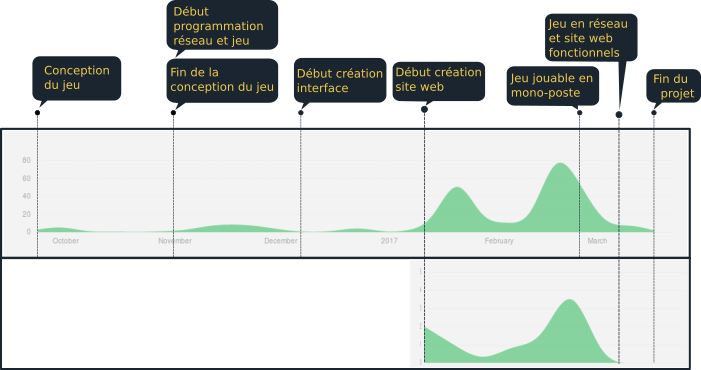
\includegraphics[scale=0.5]{Assets/gestionTemps.png}
        \caption{Gestion du temps par rapport à la courbe de \textit{commit} \textit{GitHub}}
        \label{RepTime}
      \end{center}
    \end{figure}

\end{document}
